% -----------------------------------------------------------------------------
% Resultados
% -----------------------------------------------------------------------------

\chapter{Análise e Discussão dos Resultados}
\label{chap:resultados}

\section{Provisionamento de infraestrutura}

\subsection{Configuração Inicial}

Foi utilizado para o setup inicial uma imagem customizada do Ubuntu \emph{Server} 20.04, que se valia de uma configuração prévia automatizada por meio de \href{https://cloudinit.readthedocs.io/en/latest/}{cloud-init}. Isso possibilitou a execução de todas as máquinas mantendo a uniformidade de configurações inicias de SSH, usuário e permissões de {sudo} em 2 horas, considerando que a execução foi a partir de uma única unidade de \emph{pen-drive}. A melhor opção seria disponibilizar em uma unidade de rede comum as máquinas que pudessem ser acessadas durante o boot inicial.

Para assegurar um acesso seguro a rede do Winet foi selecionado um computador para servir como \emph{load balancer} em rede privada e \emph{bastion host} para acesso externo. Nesta configuração local foi realizada a instalação de um agente de tunelamento reverso de rede \href{https://ngrok.io}{ngrok} para expor a porta 22 em um endpoint com IP público, na qual uma comunicação SSH poderia ser estabelicida mediante a chave adequada. Essa configuração foi necessária para agilizar o desenvolvimento do provisionamento de segurança, enquanto um usuário de VPN não foi provisionado, e como a solução é semelhante a um tunelamento reverso de porta, em um endpoint efêmero, as configurações de rede da UFMG não forma expostas e pouco risco foi acrescido. 


\begin{figure}[!ht]
    \centering
    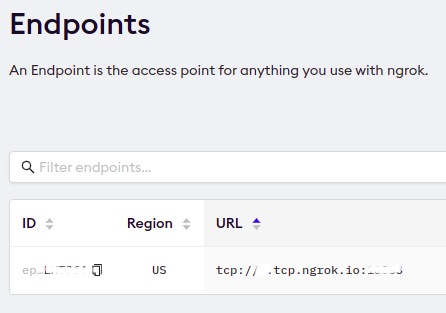
\includegraphics[width=0.5\textwidth]{04-figuras/ngrok.png}
    \caption{Ngrok Endpoint}
    \label{fig:ngrok}
\end{figure}

\begin{figure}[!ht]
    \centering
    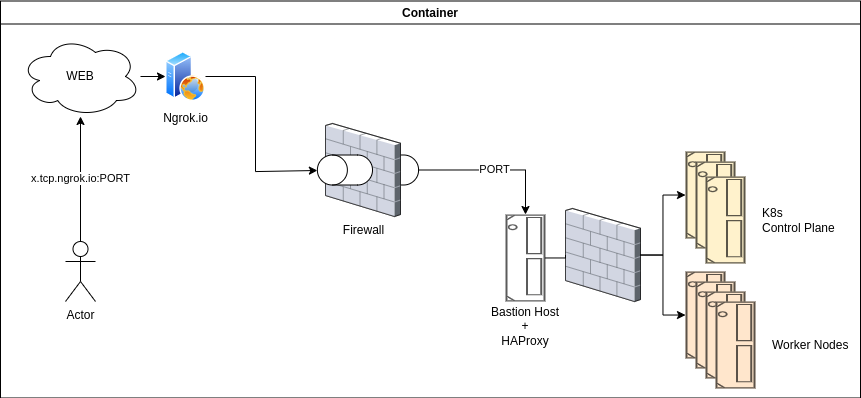
\includegraphics[width=0.8\textwidth]{04-figuras/ngroktcp.png}
    \caption{Funcionamento do Ngrok}
    \label{fig:ngroktcp}
\end{figure}

Juntamente a essa configuração foram realizadas as seguintes configurações de segurança básicas:

\begin{itemize}
    \item instaladas fail2ban com throtlle 3 requisições falhas por minuto, limitando ataques \emph{brute-force} na porta SSH;
    \item foi desabilitado login root;
    \item foi desabilitada login por com senha;
    \item habilitado trafego na porta 22 de qualquer IP; e
    \item habilitado trafefo em qualquer porta de IPs dentro da faixa de CIDR da subnet
\end{itemize}



\subsection{Configurações dos computadores }
Uma vez que uma conexão SSH foi estabelicida e o \emph{firewall} todo  \emph{cluster} foi configurado utilizando o gerenciador de configurações (CMS) Ansible\textregistered. A configuração total do \emph{cluster} demora entre 20-35 minutos sendo que a configuração foi realizada mais de uma vez do zero para garantir que todo o \emph{playbook} (conjunto de configurações a serem executadas) fosse executado corretamente, considerando sua execução do início ao final e considerando a máquina sem nenhuma das configurações até seu estado de pronta. A execução idempotente (i.e operação realizada mais de uma vez sem que o resultado se altere) não foi alcançada para as configurações dos nós mestres devido à restrição de tempo e número de etapas a serem configuradas. Na figura \ref{fig:ansibleflow} pode-se observar o diagrama de fluxo de execução lógica do \emph{playbook}, porém essa não é a divisão modular do código, que é apresentado na forma de \emph{roles}. 

\begin{figure}[!ht]
    \centering
    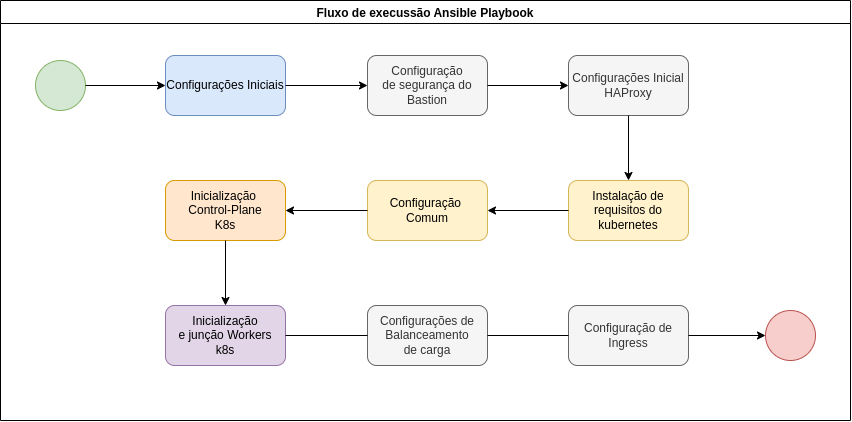
\includegraphics[width=\linewidth]{04-figuras/ansibleflow.png}
    \caption{Fluxo de execução do Ansible Playbook}
    \label{fig:ansibleflow}
\end{figure}

A formulação do inventário (que no Ansible\textregistered\ refere-se a relação de máquinas identificadas e/ou agrupadas, onde é possivel especificar configurações e variáveis, para as mesmas) considera que os computadores a serem configurados estejam na mesma rede do bastion, sendo que toda a configuração passa por ele, garantindo assim a segurança da execução apenas para outros computadores, para os quais possa ser estabelecida conexão a partir dele. Esse inventário também divide em grupos as máquinas, podendo assim ser executado o playbook novamente para novas maquinas a serem adicionadas ao \emph{cluster} , que garante o recrutamento estático de novos nós para comporem o cluster, e virtualmente podendo chegar no limite de rede no qual os nós do \emph{cluster} estão agrupados. Para garantir a correta execução o inventário pode ser referenciado explicitamente durante a execução desde que tenha o mesmo formato do disponibilizado no repositório.

\subsection{Configurações de infra do cluster}
Duas ferramentas de vasto uso na configuração de infraestrutura e também do Kubernetes\textregistered\ foram utilizadas para garantir a gestão do provisionamento e configurações das aplicações que estão sendo executadas no \emph{cluster}. 

Terraform\textregistered\ é uma ferramenta de infraestrutura como código que permite definir recursos em arquivos de configuração legíveis. Essa ferramenta possibilita o provisionamento e gerenciamento de toda a infraestrutura por ela definida e seu ciclo de vida (provisionamento, alterações e decomissionamento). Essa ferramenta possui recursos que garantem a execução respeitando relações de dependência entre recursos, sejam elas diretas ou não.

Helm\textregistered\ é uma ferramenta de gerenciamento de pacotes para Kubernetes\textregistered\, tendo nela contida todas as configurações necessárias para configuração do \emph{cluster} com uma dada aplicação. 

O provisionamento de novas cargas de trabalho e \emph{stacks} de processamento de dados foram realizados combinando o uso de Terraform\textregistered,\ que garantiu a correta gestão do estado dos recursos provisionados no \emph{cluster}, com o Helm\textregistered\, que garantiu a correta configuração das aplicações configuradas no \emph{cluster}. Essa combinação garantiu a máxima eficiência, gerenciando as dependências entre recursos e aplicações durante o tempo de execução, garantindo a imutabilidade dos recursos provisionados, o que diminui o \emph{drift} ou desvio de configurações, minimizando anti padrões como \emph{snowflake}\cite{snowflakeanti}.

\subsection{Gestão de armazenamento no \emph{cluster}}
Para gerenciar recursos que necessitam de persistência de dados neles contidos no Kubernetes\textregistered\ é necessário utilizar um conjunto de objetos de configuração específicos. Uma vez que container é um recurso efêmero, é necessário explicitar \textbf{o que} e \textbf{como} persistir dados que não devem ser perdidos quando o mesmo é desalocado no \emph{cluster}. 

Para isso existe um conjunto próprio de API (\emph{application programming interface}) para persistir um conjunto de dados de um ou mais containers no Kubernetes\textregistered. \emph{PersistentVolume (PV)} e \emph{PersistentVolumeClaim (pvc)} são dois objetos de APIs que gerenciam persistência dinâmica de dados utilizando \emph{StorageClass}. PV é um recurso que possui um ciclo de vida diferente e individual de um pod. PVC é uma solicitação de armazenamento dentro do \emph{cluster}, que pode solicitar a um PV ou diretamente a um StorageClass (perfis de volumes). Sendo que no segundo, algumas configurações sobre politicas de acesso e qualidade de serviço podem ser previamente especificadas, deixando o requerente responsável apenas por configurações mais simples, como tamanho do volume necessário. Para configurações de volumes que utilizam protocolos especificos de sistema de arquivos, como NFS (\emph{network file system}), pode se utilizar uma API especifica chamada \emph{container storage interface}(CSI) que abstraí especificidades de como um volume deve ser provisionado e como um container deve se anexar a ele.

StorageClass é a forma mais recomendada para gerenciamento de CSI para disponiblizar volumes compartilhados no \emph{cluster} de Kubernetes\textregistered, porém em \emph{clusters }\emph{bare-metal} não existem muitas opções de \emph{provider} CSI que não necessitem de um software ou ainda hardware específico, como no caso de SANs (\emph{StorageAreaNetwork}) específícos. Sem CSI, as chamadas de \emph{filesystem} que são executados pelos containers que alocam PVC (\emph{persistent volumes claim}) podem incorrer em erros o que resulta na perda de dados ou ainda em erros de IO (\emph{input output}). 


Tendo como premissa que alguns volumes devem estar disponíveis para o cluster, e não ao container, não é possivel utilizar PV (persistent volumes) ou StorageClasses que sejam locais. Ou seja, que não disponibilizem aquele volume ao \emph{cluster} como um todo, uma vez que um pod ao ser encerrado por qualquer motivo pode ser alocado novamente em outro nó do cluster, que não possuirá qualquer registro da informação escrita anteriormente. 

Com isso, resumimos a duas alternativas abertas: Ceph e NFS. Ambos os protocolos possuem CSI. Primeiramente, optou-se por utilizar o Ceph, uma vez que esse protocolo possibilitaria o uso de toda a capacidade de armazenamento do \emph{cluster} de forma compartilhada, e com isso somaria-se os volumes disponiveis localmente, podendo resultar em um volume elástico que aumentaria toda vez que um nó fosse adicionado ao cluster, somando a capacidade de armazenamento do \emph{cluster} como um todo. 

Após algumas tentativas de implementação, o funcionamento correto e esperado do driver não foi alcançado. E mesmo sendo a opção mais indicada, tendo um grau de complexidade que extrapolou o tempo disponível foi substituído pelo driver NFS, que garante a disponibilidade de volumes compartilhados, mas é baseado apenas no volume local do servidor que o provê. Mesmo tendo menos benefícios, ainda atende o propósito de volumes compartilhados, e pode ser usado em uma estratégia \emph{mesh}, que garantiria uma soma de volumes entre os nós do cluster, mas que precisaria ser adaptado para ser disponiblizado como um pool de storageclasses, também fugindo do intento desse trabalho.

Por fim, visando a possivel substituição do servidor NFS, por um NAS (\emph{Netware Area Storage}) que é uma solução de hardware específico ou genérico (configurável) e, portanto, sendo mais viável do ponto de vista econômico (preço/volume). Vale ressaltar que, o menor custo vem com problemas de latência, o que pode prejudicar o desempenho de soluções de processameto de dados que sejam intensivos em leitura e escrita de dados, especialmente o segundo.

Para tornar a solução viável em termos de complexidade de configuração, disponiblidade de hardware e custo, optou-se por usar o servidor bastion e \emph{load balancer} como também o servidor de NFS. Como o número de requisições realizadas no \emph{cluster} ainda não é tão grande, uma vez que a maior parte das requisições serão internas e de comandos, não foi mapeado como um risco de desempenho, mas tornando o uso mais intenso do cluster, seria recomendado isolar a função de \emph{server} de NFS para um NAS ou servidor específico.

\section{Disponibilização das imagens de container}

Diversas dependências para a execução das tarefas e logo após a exploração visual e análise dos dados coletados pela orquestração devem ser incorporadaa às imagens base utilizadas para o Airflow e também Jupyter. Para controlar a entrega dessas imagens e disponibilizá-las para o servidor, foi publicado em um repositório de imagens publica, com credenciais que expiravam em 12 horas. Essas imagens utilizaram uma estratégia tag para \emph{release} associada ao \emph{commit message} no repositório do git, podendo assim recuperar versões específicas e rastrear mudanças que possivelmente alteraram o comportamento esperado dos containers que as utilizarem. 

Essa tag era então substituída por meio de variáveis no Terraform e assim utilizadas para configuração dos recursos durante o tempo de deploy das aplicações com as novas tags. Essa estratégia garante um fluxo auditável de mudanças e preconiza a imutabilidade, uma premissa para uso de infraestrutura como código. 

\section{Orquestração do processamento}
Para orquestrar tarefas dentro do \emph{cluster} garantindo a execução de atividades que tenham início, meio e fim, com alguma relação de dependência entre as atividades executadas, é necessário a utilização de uma aplicação capaz de orquestrar tarefas, i.e. gerenciar fluxos de trabalho. Nesse trabalho a ferramenta utilizada foi o Apache Airflow\textregistered.  Essa ferramenta gerencia atividades utilizando um grafo direcional acíclico (DAG) semelhante ao Apache Spark\textregistered. Essas atividades ou tarefas serão aqui chamadas de \emph{tasks}. Essas \emph{tasks} e suas dependências são definidas em Python (uma linguagem de programação interpretada e de tipagem dinânmica) e o Airflow gerencia o agendamento (scheduler) e a execução (executor). A execução de uma DAG pode ser por meio de eventos ou agendamento (e.g. diariamente, por hora etc.).

A configuração do processo de ETL para ingestão dos dados do banco de medicamentos industrializados foi desenhado de acordo com o diagrama de fluxo da Figura \ref{fig:diagramafluxo} e implementado  de acordo com a Figura \ref{fig:airflowdag}.

\begin{figure}[!ht]
    \centering
    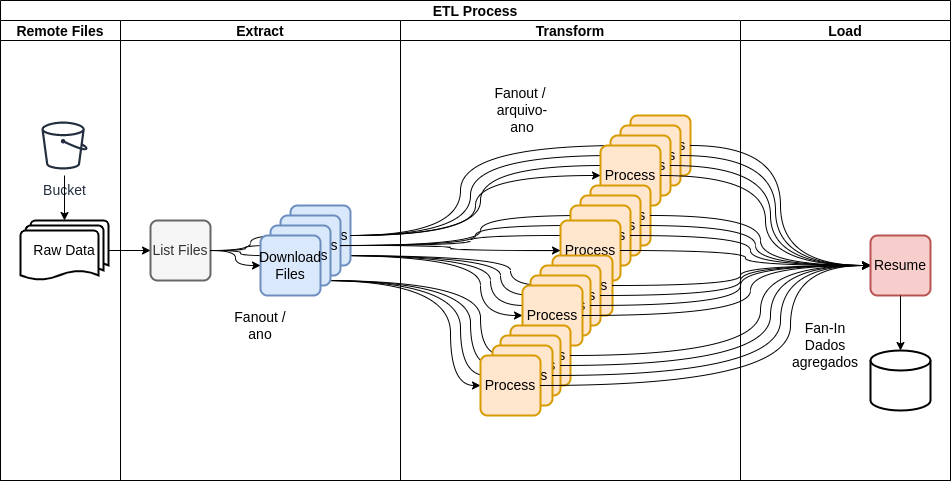
\includegraphics[width=0.8\linewidth]{04-figuras/flow-7.png}
    \caption{Airflow - Diagrama de Fluxo}
    \label{fig:diagramafluxo}
\end{figure}

\begin{figure}[!ht]
    \centering
    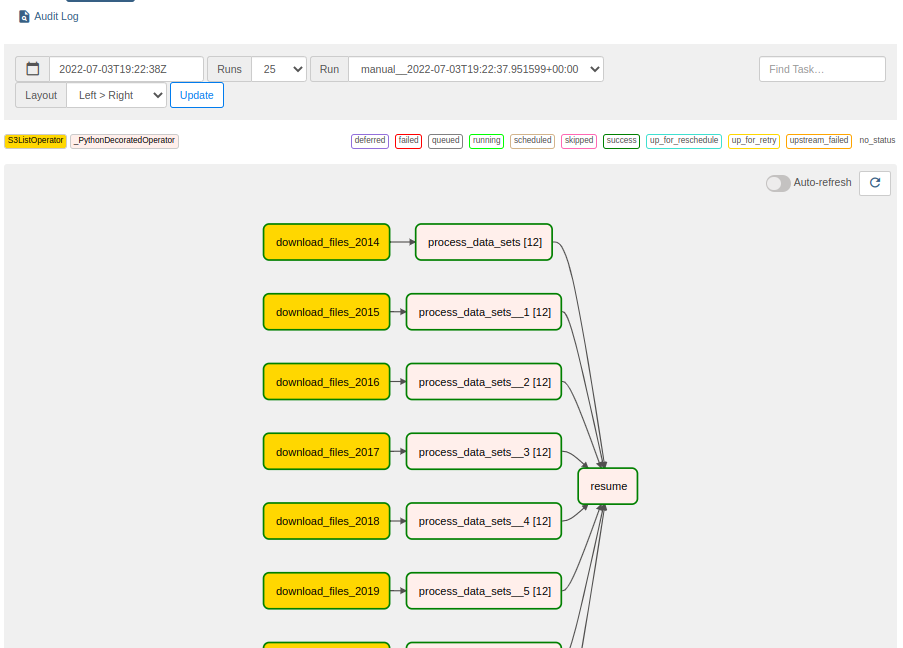
\includegraphics[width=0.8\linewidth]{04-figuras/graph_execution.png}
    \caption{ETL DAG}
    \label{fig:airflowdag}
\end{figure}

Para entender melhor a execução desse fluxo de trabalho é necessário entender como se dão as sequências de chamadas entre os componentes do Airflow. Na Figura \ref{fig:airflowsequence} pode-se visualizar o diagrama de sequência onde cada life-line é um componente da aplicação, sendo que o scheduler, o trigger, o webserver são objetos de deployment dentro do kubernetes.

\begin{figure}[!ht]
    \centering
    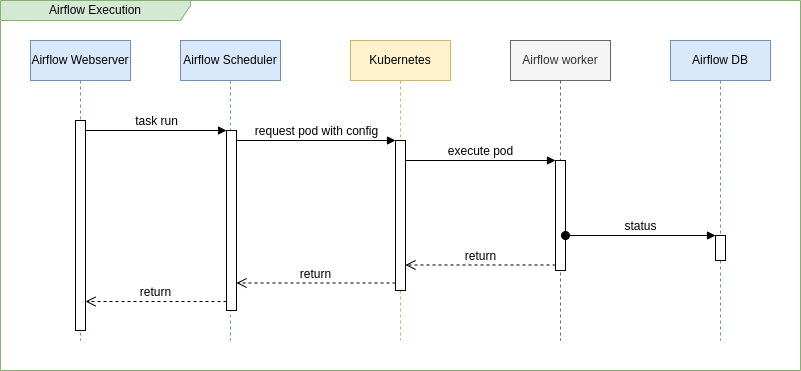
\includegraphics[width=0.8\linewidth]{04-figuras/airflow_sequence.png}
    \caption{Airflow - Diagrama de Sequência}
    \label{fig:airflowsequence}
\end{figure}

Objetos de deployment controlam objetos de replicaset que apenas controlam a quantidade de objetos pod que serão executados a partir de um modelo de configuração. Esse modelo, entre outras configurações, especifica memória, cpu, volumes, imagem de container etc. Tendo dito isso, também é necessário descrever o worker. Airflow \emph{Worker} nada mais são que os componentes que de fato executam uma \emph{task} especificada na DAG. Nesse trabalho, utilizamos o KubernetesExecutor para provisionar cada nova \emph{task} executada no \emph{cluster} em um novo pod, com recursos definidos na configuração da task, o que fica especificado em código python. 

A configuração da \emph{task} e como ela deve ser executada é passada a um modulo do Airflow \emph{Scheduler} chamado executor. O Airflow possui diversos tipos de executors. Mais comumente utliza-se o CeleryExecutor, porém para garantir que o \emph{cluster} tenha alocação das pods dinamicamente optou-se pelo KubernetesExecutor. Esse componente nada mais é que um serviço que realiza chamadas de API para o provisionamento de pods que por sua vez executaram a task.


Apesar de não representada, há uma etapa anterior, um \emph{operator} que lista os anos disponiveis para criação de grupos de \emph{mapper} de tarefas dinâmicas, é um \emph{fan-out} de duas etapas, lançando os arquivos que irão listar anos disponíveis em bucket S3 na AWS, outro que listará os arquivos disponíveis de cada ano e seu download.

Na etapa de processamento seguinte, os dados são carregados desses arquivos em memória, em um \emph{dataframe} do {pandas} (biblioteca python). Pelo tamanho dos arquivos, não é possivel fazer o carregamento de uma só vez e por tanto a opção de chunks foi usada - isso particiona os dados para garantir o processo por partes. Essa opção garante que diversas tarefas sejam executadas em parelelo sem sobrecarregar o \emph{cluster} ou mesmo causar eventos de OOM (\emph{out of memory}), fazendo assim com que a tarefa entre na fila de \emph{retry}.

O ponto de configuração dos containers foi de 1vCPU e 2GB de RAM para processar arquivos entre 0.5-0.7GB de dados por vez, como a tabela de escrita dos dados processado no PostgreSQL era a mesma para garantir a consolidação dos dados, o pipeline de execução de cada tarefa ficava entre entre 4 e 12 minutos desde o momento de início do \emph{download} até o completo carregamento em banco. Como a operação de escrita em banco também é uma atividade restrita, ou seja, não permite duas escritas simultâneas, esse com certeza era um ponto de restrição do fluxo de dados. A possivel solução para esse gargalo era a escrita dos dados pré-processados em tabelas distintas e em um passo seguinte a consolidação em tabela única. Porém, para manter a estrutura de um ETL simples e validar o processamento no cluster, não foi necessário realizar essas etapas de otimização. 

Mencionadas as limitações ja observadas, é necessário indicar mais uma importante restrição: o banco também está sendo executado no \emph{cluster} com 1,5GB de RAM e 0.3 vCPU, sendo um recurso compartilhado entre diversos outros recursos do \emph{cluster} por ter mais de um banco na mesma instância. E ainda utilizando CSI de NFS, que como mencionado anteriormente adiciona latência e conhecidamente não performa muito bem em usos intensos de escritas.

\begin{figure}[!ht]
    \centering
    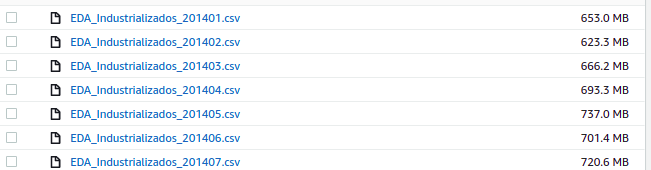
\includegraphics[width=0.8\linewidth]{04-figuras/s3_size.png}
    \caption{S3 armazenamento dos dados}
    \label{fig:s3_storage}
\end{figure}


Considerando o tamanho e tempo médio de execução das atividades podemos inferir que:
\begin{itemize}
    \item o tempo de execução total dessas tarefas de forma serial, seria de aproximadamente $8 min\ *\ 90 arquivos = 720min$ para importar todos os arquivos
    \item mesmo com as execuções simultâneas limitadas a 12, não utilizamos 50\% do cluster, como demonstrado na Figura \ref{fig:consumocluster}
\end{itemize} . 


\begin{figure}[!ht]
    \centering
    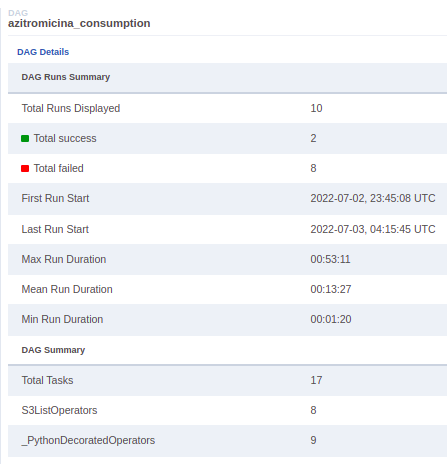
\includegraphics[width=0.5\linewidth]{04-figuras/report_execution_summary1.png}
    \caption{Relatório de execução}
    \label{fig:report}
\end{figure}

É possivel avaliar que a sobreposição de tarefas é gerenciada pelo Airflow mantendo a restrição de 12 execuções por vez, como demonstrado na Figura \ref{fig:gantt}. Essa configuração foi limitada diretamente no Airflow durante o provisionamento, utilizando variáveis de ambiente. Essa restrição foi utilizada para restringir o número de escritas simultâneas que poderiam ocorrer no banco de dados que armazena a saída de cada uma das tarefas. Caso o numero de concorrentes fosse máximo, duas coisas poderiam ocorrer: 1) o tempo para finalizar cada \emph{task} poderia extrapolar o limite de tempo definido para cada \emph{task} ser executada ou 2) o banco poderia ser sobrecarregado de requisições demorando ainda mais para inserir os dados em tabela, uma vez que teria que gerenciar as requisições de inserção simultâneas. 

\begin{figure}[!ht]
    \centering
    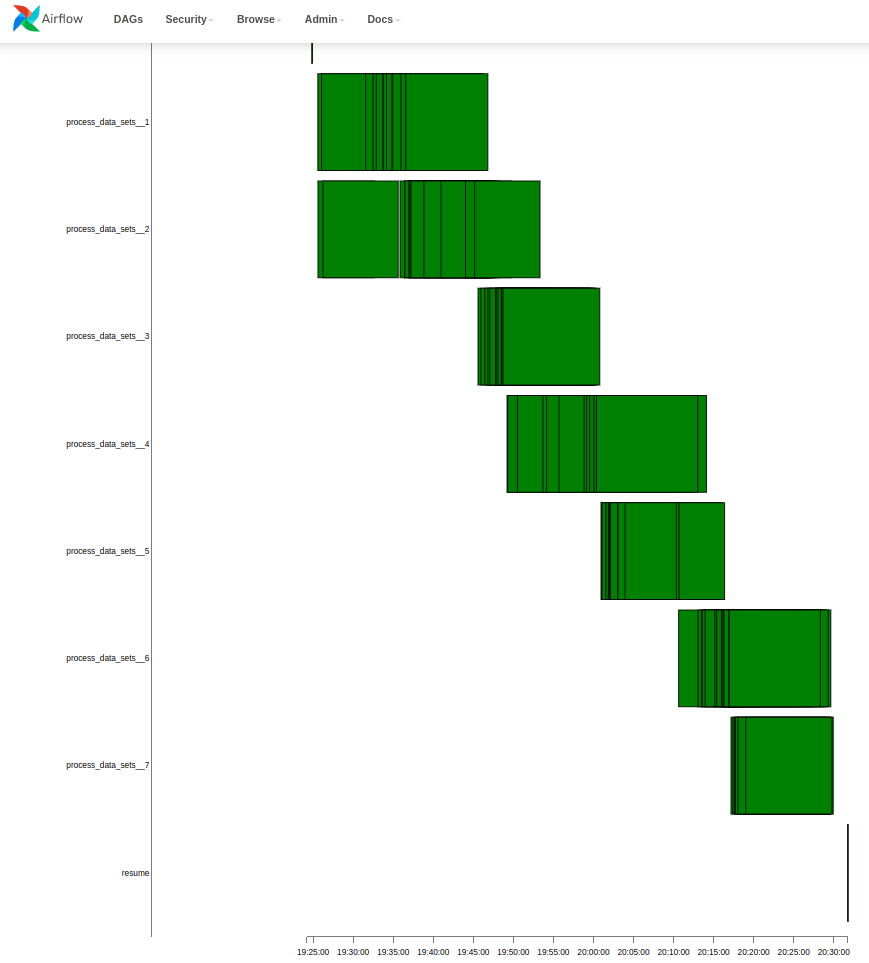
\includegraphics[width=0.7\linewidth]{04-figuras/gantt.png}
    \caption{Grafico de Gantt da orquestração}
    \label{fig:gantt}
\end{figure}

Porém, o tempo total gasto foi de 53 min, segundo a Figura \ref{fig:report}. Isso representa 55\% do tempo esperado, mesmo considerando as restrições de desempenho citadas anteriormente.

Pode se inferir que o número de execuções simultâneas representavam 24vCPUs e 48GB de memória por limite de tarefas em execução, representando um servidor que sozinho custaria entre 20 e 40 mil reais, e nesse trabalho utilizou-se apenas máquinas que não estavam sendo utilizadas do DCC UFMG.

\section{Desempenho do cluster}
Devido as restrições colocadas para execuções simultâneas no cluster, garantimos que o \emph{cluster} não fosse completamente utilizado, o que permitiria o seu uso para outras aplicações que viessem a ser executadas simultaneamente. Esse resultado atende a um dos objetivos específicos desse trabalho. Como mostrado na Figura \ref{fig:consumocluster} as atividades do \emph{cluster} não ultrapassam em nenhum momento durante a execução do processo de importação e processamento dos dado. Essa avaliação utilizando o método USE de monitoramento permite analisar problemas de desempenho e identifica-los de maneira mais direta.

Para avaliar esse gráfico precisa-se identificar que as linhas amarela, azul e verde, representam os nós que pertencem ao \emph{control-plane}, ou seja os nós que realizam as atividades de controle do \emph{cluster} e parte de seu monitoramento. Esse monitoramento diz respeito apenas aos objetos que estão sendo supervisionados, ou seja, sob avaliação do control-manager e \emph{scheduler} por meio do apiserver. As demais linhas são nós workers, que efetivamente executam as cargas de trabalho e visivelmente tem sua capacidade mais exigida durante o processo de importação e processamento dos dados. 

Para a \emph{task} de download, primeira etapa do fluxo de trabalho realizado no Airflow, é possivel notar que o processo demanda mais escrita e leitura de disco e também possui maior atividade de rede e memória. Isso se deve ao fato de estar realizando tanto o download dos arquivos da fonte de dados, como também escrevendo o arquivo em disco. Após essa tarefa o uso de memória e disco se tornam ciclicos, essa ciclicidade se deve ao fato de que apenas 12 tarefas podem ser executadas por vez, como apresentado anteriomente nesse capítulo. Como todas as tarefas subsequentes escrevem o resultado em disco após a finalização pode-se observar que o resultado de escrita em disco e rede também é elevado, porém a diferença nessa etapa é que a escrita apesar de ser em disco, utiliza o volume de dados do container com CSI-NFS. Sendo um protocolo de arquivos de sistema em rede, esses arquivos são temporariamente escritos em disco e logo retransmitidos ao NFS \emph{server} o que gera o tráfego de rede elevado no cluster, a semelhança do primeiro processo de download simples dos arquivos. 

Para reforçar essa observação sobre a execução do processo, avalia-se o monitoramento dos nós realizado pelo control plane, que enxerga a capacidade total do cluster, ao invés de seus nós na figura \ref{fig:cluster}. Já na figura \ref{fig:container} pode-se observar o comportamento sobreposto da utilização percentual de memória e cpu dos pods que executam as tarefas em relação ao cluster.

\begin{figure}[!ht]
    \centering
    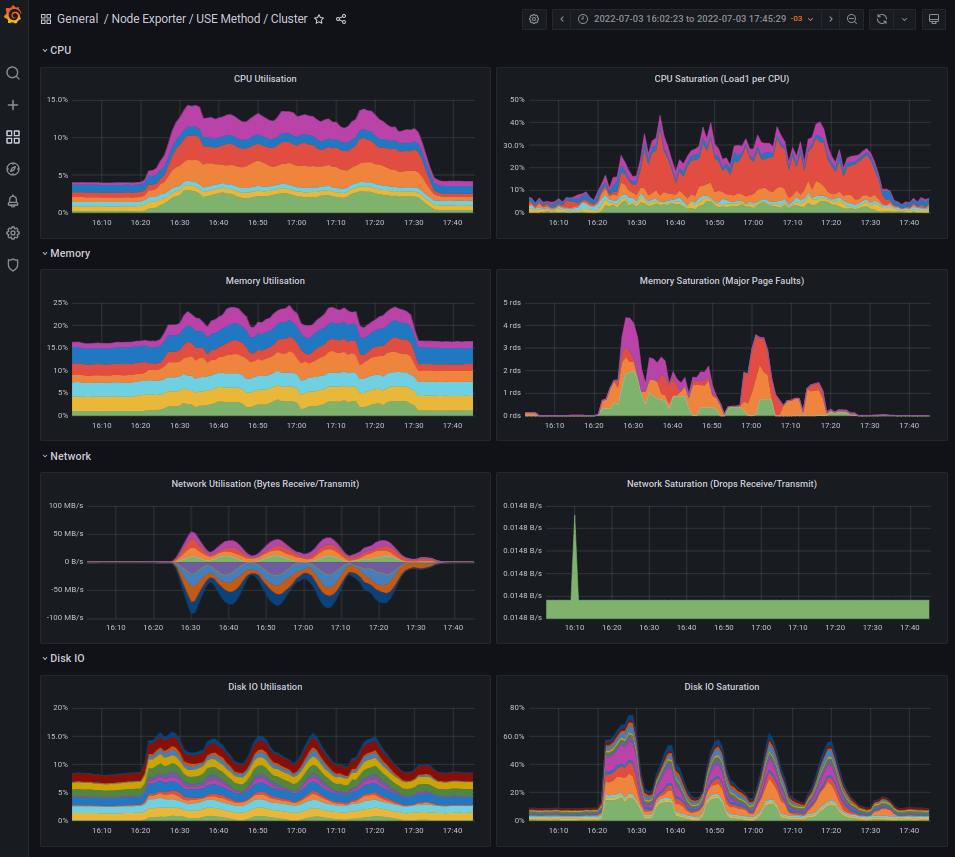
\includegraphics[width=0.85\linewidth]{04-figuras/Usemethod.png}
    \caption{Método USE monitoramento de hardware}
    \label{fig:consumocluster}
\end{figure}

\begin{figure}[!ht]
    \centering
    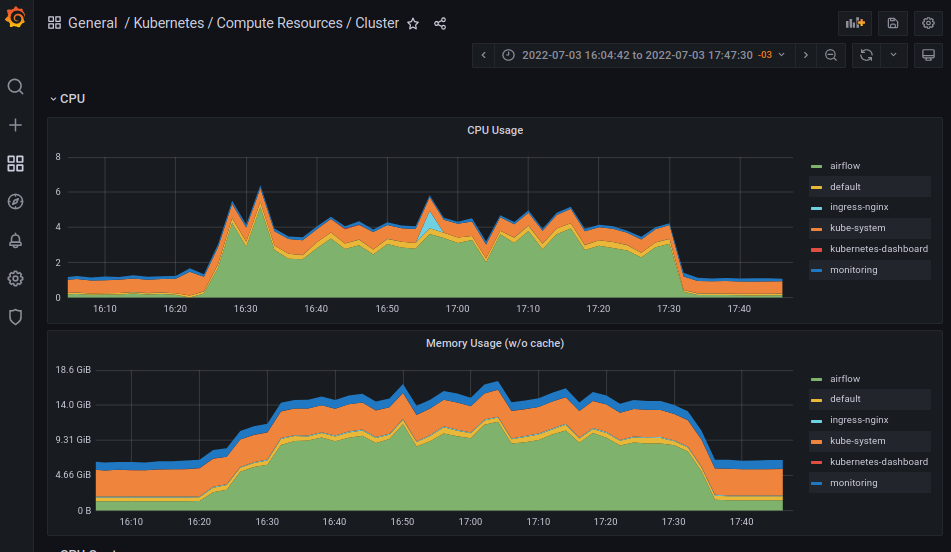
\includegraphics[width=0.85\linewidth]{04-figuras/cluster_usage.png}
    \caption{Monitoramento do \emph{cluster} pelo Control-Plane}
    \label{fig:cluster}
\end{figure}

\begin{figure}[!ht]
    \centering
    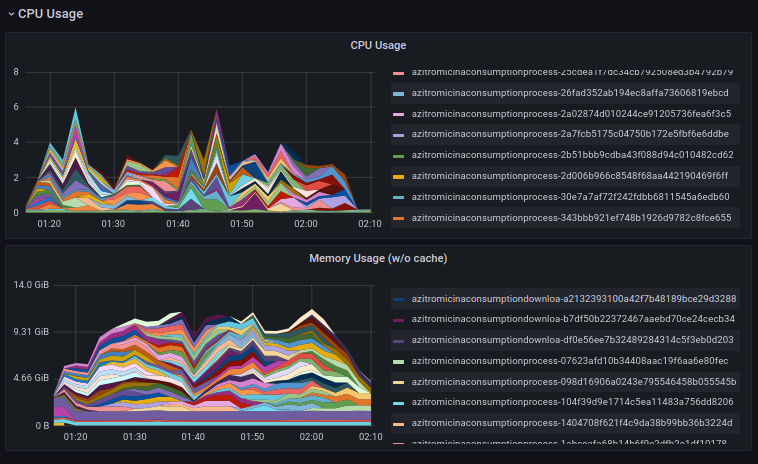
\includegraphics[width=0.85\linewidth]{04-figuras/etl_2_usage.png}
    \caption{Perfil da aplicação - Utilização dos pods de processamento em relação ao cluster}
    \label{fig:cluster}
\end{figure}

A diferença de métricas possibilita ter uma visão mais holistica de como a aplicação esta utilizando o \emph{cluster} em si, e também possibilita validar alguns pontos. 
\begin{itemize}
    \item O número de atividades em paralelo poderia ser aumentado, garantido assim melhor utilização do cluster, porém seria necessário alterar a lógica de processamento para escrever em tabelas individualizadas no banco de dados, e resumi-las na última etapa do processo. 
    \item Protocolos de rede que garantissem o compartilhamento de dados entre os discos dos nós (como o Ceph) poderiam representar ganhos significativos, não sendo necessário trafegar todo o dado para fora do nó, quando houvesse uma escrita em disco.
    \item O processo de fanout utilizado 
\end{itemize}

\section{Análise de dados}
Todas as análises foram executas em um Jupyter notebooks provisionado no cluster.

Um total de 95.345.640 prescrições de azitromicina foram atendidas em farmácias e drogarias do Brasil, entre 2015 e 2021. A maioria dos pacientes para os quais foi dispensado o medicamento era do sexo feminino (53,62\%), com média de idade de 32,75 (± 2,04). Entre as regiões com maior venda de azitromicina destacam-se as regiões Sudeste (47,44\%) e Sul (22,47\%) e entre as UF, destacam-se São Paulo (24,76\%), Minas Gerais (13,17\%) e Rio Grande do Sul (12,49\%) Tabela \ref{table:base_desc}

\begin{table}[!htbp]
    \centering
    \begin{tabular}{llll}
    \hline
    \multicolumn{2}{l}{\multirow{2}{*}{\textbf{Características}}} & \textbf{n} & \textbf{\%} \\ \cline{3-4} 
    \multicolumn{2}{l}{}                                          & 95345640   & 100         \\ \hline
    \multicolumn{2}{l}{\textbf{Sexo do paciente}}                 &            &             \\
                         & Feminino                               & 50051932   & 53,62       \\
                         & Masculino                              & 45293708   & 46,38       \\
    \multicolumn{2}{l}{\textbf{Região}}                           &            &             \\
                         & Centro Oeste                           & 8325772    & 8,73        \\
                         & Nordeste                               & 15311389   & 15,44       \\
                         & Norte                                  & 5050278    & 5,3         \\
                         & Sudeste                                & 45232822   & 47,44       \\
                         & Sul                                    & 21425379   & 22,47       \\
    \multicolumn{2}{l}{\textbf{Unidade Federativa}}               &            &             \\
                         & Acre                                   & 235293     & 0,25        \\
                         & Alagoas                                & 587010     & 0,62        \\
                         & Amapá                                  & 251408     & 0,26        \\
                         & Amazonas                               & 541218     & 0,57        \\
                         & Bahia                                  & 3672405    & 3,85        \\
                         & Ceara                                  & 2545617    & 2,67        \\
                         & Distrito Federal                       & 1205841    & 1,26        \\
                         & Espírito Santos                        & 1704011    & 1,79        \\
                         & Goiás                                  & 5007864    & 5,25        \\
                         & Maranhão                               & 1414456    & 1,48        \\
                         & Mato Grosso                            & 1068418    & 1,12        \\
                         & Mato Grosso do Sul                     & 1043649    & 1,09        \\
                         & Minas Gerais                           & 12552967   & 13,17       \\
                         & Pará                                   & 2640661    & 2,77        \\
                         & Paraíba                                & 2207241    & 2,31        \\
                         & Paraná                                 & 5818312    & 6,1         \\
                         & Pernambuco                             & 1823847    & 1,91        \\
                         & Piauí                                  & 861105     & 0,9         \\
                         & Rio de Janeiro                         & 7372345    & 7,73        \\
                         & Rio Grande do Norte                    & 1653179    & 1,73        \\
                         & Rio Grande do Sul                      & 11911733   & 12,49       \\
                         & Rondônia                               & 693489     & 0,73        \\
                         & Roraima                                & 199669     & 0,21        \\
                         & Santa Catarina                         & 3695334    & 3,88        \\
                         & São Paulo                              & 23603499   & 24,76       \\
                         & Sergipe                                & 546529     & 0,57        \\
                         & Tocantins                              & 488540     & 0,51        \\ \hline
    \end{tabular}
    \caption{Características das prescrições de azitromicina atendidas em farmácias e drogarias, Brasil, 2014-2020.}
    \label{table:base_desc}
    \end{table}

    No período de 6 anos, em números absolutos, o número de prescrições de azitromicina, no Brasil, aumentou de 13.421.249 prescrições em 2014 para 17.735.901 prescrições em 2020, representando um aumento de 32,1\%. Considerando o crescimento da população, isso representa um aumento na taxa de prescrição de azitromicina de 66,2 para 83,8 prescrições por 1.000 habitantes, em todo o período Tabela \ref{table:base_region}. 


    \begin{table}[!htbp]
        \centering
    \begin{tabular}{llrr}
    \hline
    \multicolumn{2}{l}{\multirow{2}{*}{\textbf{Localidade}}} & \multicolumn{2}{l}{\textbf{Taxa prescrição / $10^4$ hab}} \\ \cline{3-4} 

    \multicolumn{2}{l}{}                                     & \textbf{2014}              & \textbf{2020}              \\ \hline
    \multicolumn{2}{l}{\textbf{Brasil}}                      & 66,2                       & 83,8                       \\
    \multicolumn{2}{l}{\textbf{Unidade Federativa}}          &                            &                            \\
                      & Acre                                 & 30,2                       & 71,9                       \\
                      & Alagoas                              & 20,5                       & 42,8                       \\
                      & Amapá                                & 36,5                       & 79,2                       \\
                      & Amazonas                             & 13                         & 38                         \\
                      & Bahia                                & 46,3                       & 51,5                       \\
                      & Ceara                                & 23,8                       & 38,3                       \\
                      & Distrito Federal                     & 52,7                       & 96,9                       \\
                      & Espírito Santos                      & 49,6                       & 97,8                       \\
                      & Goiás                                & 133,2                      & 116,1                      \\
                      & Maranhão                             & 19,6                       & 31,1                       \\
                      & Mato Grosso                          & 31,3                       & 73,5                       \\
                      & Mato Grosso do Sul                   & 49,4                       & 79,2                       \\
                      & Minas Gerais                         & 66,2                       & 149,2                      \\
                      & Pará                                 & 30,6                       & 49,4                       \\
                      & Paraíba                              & 145,2                      & 101,7                      \\
                      & Paraná                               & 57,8                       & 129,2                      \\
                      & Pernambuco                           & 26,2                       & 39,3                       \\
                      & Piauí                                & 116,8                      & 33,7                       \\
                      & Rio de Janeiro                       & 44,1                       & 76,2                       \\
                      & Rio Grande do Norte                  & 50                         & 106,7                      \\
                      & Rio Grande do Sul                    & 137,6                      & 97,4                       \\
                      & Rondônia                             & 37,5                       & 109,4                      \\
                      & Roraima                              & 37,3                       & 99,8                       \\
                      & Santa Catarina                       & 61,3                       & 84,5                       \\
                      & São Paulo                            & 96,6                       & 86,7                       \\
                      & Sergipe                              & 30,7                       & 58,6                       \\
                      & Tocantins                            & 34,5                       & 80,6                       \\ \hline
    \end{tabular}
    \caption{Taxas de prescrição de azitromicina atendidas em farmácias e drogarias, no Brasil, em 2014 e 2020}
    \label{table:base_region}
    \end{table}

    A maioria das UF apresentaram aumento nas taxas de prescrição de azitromicina por 1.000 habitantes, com destaque para: Minas Gerais (66,2 para 149,2 prescrições por 1.000 habitantes), Rondônia (37,5 para 109,4 prescrições por 1.000 habitantes) e Roraima (37,2 para 99,8 prescrições por 1.000 habitantes).
Considerando apenas os anos de 2019 e 2020, como períodos pré e durante a pandemia da COVID-19, respectivamente, observa-se que houve aumento nas taxas de prescrição no Brasil e em todas UF, exceto no Rio de Janeiro (87,3 para 76,2 prescrições por 1.000 habitantes) e no Rio Grande do Sul (106,6 para 97,4 prescrições por 1.000 habitantes) (Tabela \ref{table:base_region1}).
\begin{table}[!htbp]
    \centering
\begin{tabular}{llrr}
    \hline
    \multicolumn{2}{l}{\multirow{2}{*}{\textbf{Localidade}}} & \multicolumn{2}{l}{\textbf{Taxa prescrição / $10^4$ hab}} \\ \cline{3-4} 
    \multicolumn{2}{l}{}                                     & \textbf{2019}              & \textbf{2020}              \\ \hline
    \multicolumn{2}{l}{\textbf{Brasil}}                      & 59,9                       & 83,8                       \\
    \multicolumn{2}{l}{\textbf{Unidade Federativa}}          &                            &                            \\
                      & Acre                                 & 32,3                       & 71,9                       \\
                      & Alagoas                              & 23,5                       & 42,8                       \\
                      & Amapá                                & 45,9                       & 79,2                       \\
                      & Amazonas                             & 17,3                       & 38                         \\
                      & Bahia                                & 31,9                       & 51,5                       \\
                      & Ceara                                & 29,7                       & 38,3                       \\
                      & Distrito Federal                     & 57,3                       & 96,9                       \\
                      & Espírito Santos                      & 62,5                       & 97,8                       \\
                      & Goiás                                & 74,3                       & 116,1                      \\
                      & Maranhão                             & 18,5                       & 31,1                       \\
                      & Mato Grosso                          & 49,2                       & 73,5                       \\
                      & Mato Grosso do Sul                   & 56,4                       & 79,2                       \\
                      & Minas Gerais                         & 81,7                       & 149,2                      \\
                      & Pará                                 & 27,3                       & 49,4                       \\
                      & Paraíba                              & 62,3                       & 101,7                      \\
                      & Paraná                               & 66,3                       & 129,2                      \\
                      & Pernambuco                           & 27,2                       & 39,3                       \\
                      & Piauí                                & 22,1                       & 33,7                       \\
                      & Rio de Janeiro                       & 87,3                       & 76,2                       \\
                      & Rio Grande do Norte                  & 73                         & 106,7                      \\
                      & Rio Grande do Sul                    & 106,6                      & 97,4                       \\
                      & Rondônia                             & 58,8                       & 109,4                      \\
                      & Roraima                              & 38,9                       & 99,8                       \\
                      & Santa Catarina                       & 73,3                       & 84,5                       \\
                      & São Paulo                            & 68,1                       & 86,7                       \\
                      & Sergipe                              & 36                         & 58,6                       \\
                      & Tocantins                            & 44,1                       & 80,6                       \\ \hline
    \end{tabular}
    \caption{Taxas de prescrição de azitromicina atendidas em farmácias e drogarias, no Brasil, em 2019 e 2020}
    \label{table:base_region1}
    \end{table}

    Os maiores aumentos nas taxas de prescrição de azitromicina foram observados em Minas Gerais (81,7 para 149,2 prescrições por 1.000 habitantes), Paraná (66,3 para 129,2 prescrições por 1.000 habitantes), Roraima (38,9 para 99,8 prescrições por 1.000 habitantes), Rondônia (58,8 para 109,4 prescrições por 1.000 habitantes) e Goiás (74,3 para 116,1 prescrições por 1.000 habitantes). 

    Pode se observar os numero absolutos na Figura \ref{fig:presc_ano_estadp}


    Pode-se observar que o resultado é coerente quando avaliado sob a perspectiva do Tau de Kendal como descrito na Figura \ref{fig:tau}, que avalia a correlação de crescimento entre variáveis. Os estados do Amazonas, Mato Grosso, Mato Grosso do Sul, Paraná, Pará, Rio Grande do Norte, Santa Catarina e Tocantins, apresentam um alto grau de correlação de crescimento no tempo e com significância estatistica (valor p < 0.05). Apesar dos resultados para o estado de Minas Gerais descrito acima, o mesmo não apresenta significância estatistica, o que pode ser causdo pelo aumento populacional do estado, o que pode mascarar o aumento da taxa de prescrição.

    \begin{figure}[!ht]
        \centering
        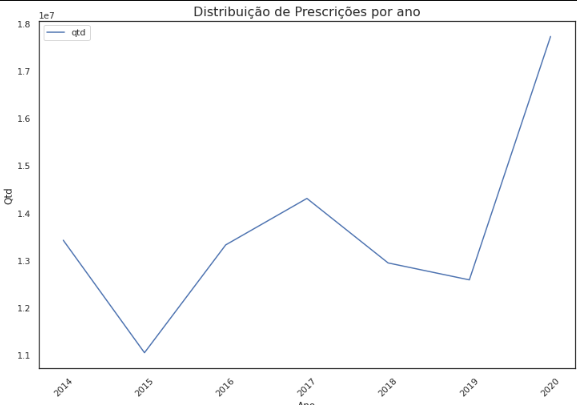
\includegraphics[width=0.8\linewidth]{04-figuras/distribuicao_presc_ano.png}
        \caption{Precrição por ano}
        \label{fig:presc_ano}
    \end{figure}
    \begin{figure}[!ht]
        \centering
        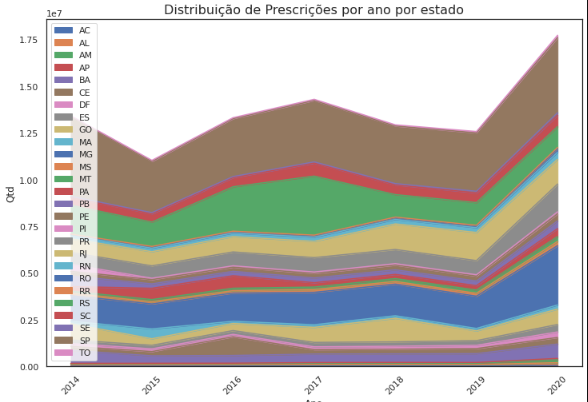
\includegraphics[width=0.8\linewidth]{04-figuras/distribuicao_presc_ano_estado.png}
        \caption{Precrição por ano por estado}
        \label{fig:presc_ano_estadp}
    \end{figure}
    \begin{figure}[!ht]
        \centering
        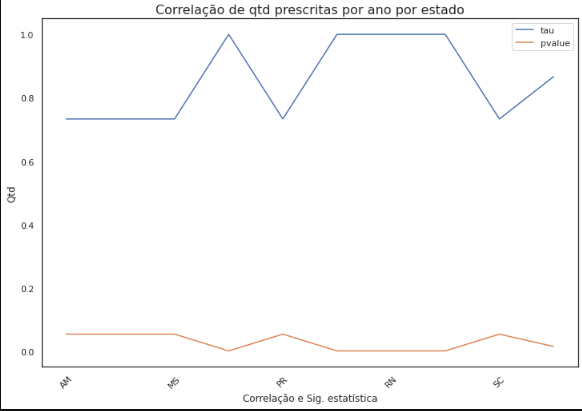
\includegraphics[width=0.8\linewidth]{04-figuras/corelaticao_estados.png}
        \caption{Avaliação de correlação de crescimento por ano por estado utilizando tau de Kendall}
        \label{fig:tau}
    \end{figure}

